\documentclass[boxes, qed]{homework}

\usepackage{xcolor,amsmath,listings}
\usepackage{graphicx}
\usepackage[backend=biber, style=mla, citestyle=authoryear]{biblatex}
\usepackage{euler}

\addbibresource{homework-9.bib}
\graphicspath{ {./images/} }

\name{Rohit Wason}
\course{Math 560}
\term{Spring 2021}
\hwnum{(\#10, Regression)}

\newcommand{\bigzero}{\mbox{\normalfont\Large\bfseries 0}}
\newcommand{\rvline}{\hspace*{-\arraycolsep}\vline\hspace*{-\arraycolsep}}
\DeclarePairedDelimiter\abs{\lvert}{\rvert}%
\DeclarePairedDelimiter\norm{\lVert}{\rVert}%

\begin{document}

\begin{problem}Given:\\
  $n=500$\\
  Mean height of the fathers, $\bar{x}=67.9$ (explanatory vaiable)\\
  Standard deviation of the height of fathers, $s_x=2.75$\\
  Mean height of the sons, $\bar{y}=68.7$ (response vaiable)\\
  Standard deviation of the height of sons, $s_y=2.83$\\
  The correlation between the heights of the sons and their fathers, $r=0.5$.
\end{problem}
\begin{solution}
  (a) Give a $99$\% prediction interval for the height of a son whose father is $70$ inches tall.\\
  Using $b_1=r(s_y/s_x)$ and $b_0=\bar{y}-b_1\bar{x}$ we have that
  $$b_1=0.5(2.83/2.75)\approx 0.5145$$
  $$b_0=68.7 - 0.5145(67.9) \approx 33.7654$$
\end{solution}

\begin{problem}
  \begin{tabular}{l|l}\hline
    Year($x$) & Kilobits($y$)\\\hline
    1971&1\\\hline
    1980&62.5\\\hline
    1987&1000\\\hline
    1993&16000\\\hline
    1998&125000\\\hline
    2000&250000\\\hline
    2002&500000\\\hline
    2004&976562.5\\\hline
  \end{tabular}
\end{problem}
\begin{solution}(a) We build the model,
  \begin{lstlisting}[backgroundcolor = \color{lightgray},language = R]
    lmKilo=lm(Kilobits~Year, data = dram)
    lmKilo$coefficients
    > (Intercept)      Year 
    > -40886934.88     20644.12
  \end{lstlisting}
  to receive the coefficients $b_0=-40886934.88, b_1=20644.12$.
  Therefore the equation of the least-square regression line is
  $$\hat{y}=-40886934.88 + 20644.12(x)$$

  (b)\begin{enumerate}
    \item Test $H_0: \beta_1=0$ vs. $H_a:\beta_1>0$
    \item Level $\alpha=0.02$
    \item Test statistic $t=\frac{b_1}{SE_{b_1}}$
  \end{enumerate}

  \begin{lstlisting}[backgroundcolor = \color{lightgray},language = R]
    SSE=sum(lmKilo$residuals^2)
    [1] 438637466614
  \end{lstlisting}

  \begin{align*}
    SSE &= \sum(y_i-\hat{y_i})^2 = 438637466614\\
    s &= \sqrt{\frac{SSE}{n-2}} = 270400\\
    s_x &= 11.6795 \implies SE_x=11.6795/\sqrt{8} = 4.129327\\
    s_y &= 347560.1 \implies SE_y=347560.1/\sqrt{8} = 122881\\
    SE_{b_1} &= \frac{s}{s_x\sqrt{n-1}}
      = \frac{270400}{4.129327(7)}
      \approx 9355
  \end{align*}
  
  Therefore the test statistic, 
  $$t=\frac{20644.12}{9355} \approx \boxed{2.2067}$$

  The critical value at $\alpha=0.02, df=n-p-1=6$ such that $P(T>t^*)=\alpha$.
  $$\implies \boxed{t^*=2.612}.$$

  Since $t>t^*$, we \textbf{fail to reject $H_0$}.\\

  (c) Scatterplot of Year-Kilobits, with R-line:\\
  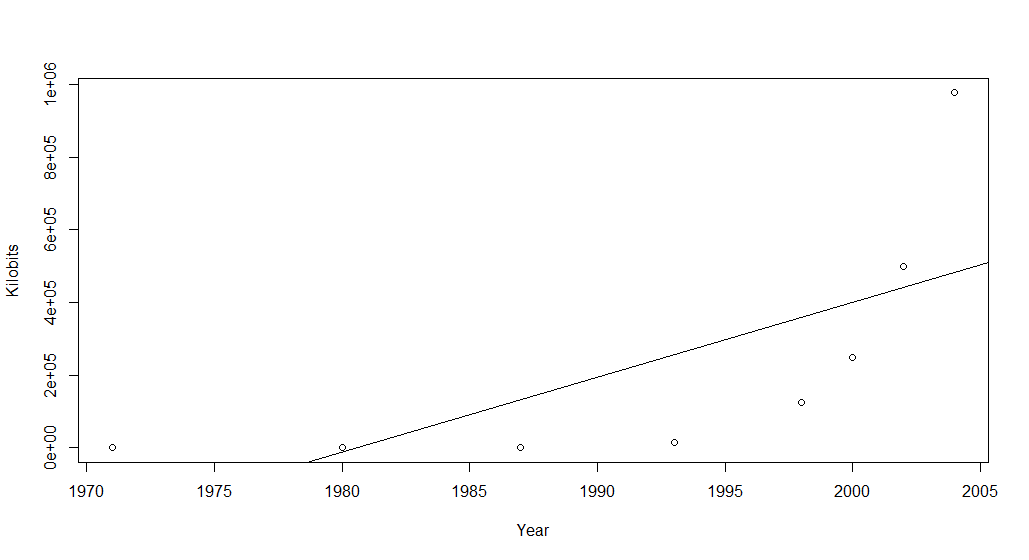
\includegraphics[scale=.5]{hw-10-2-c}
  
  (d) To find the equation of the least-squares regression line for modeling $ln(y)$ 
  as a linear function of $x$ we build a different model,\\
  \begin{lstlisting}[backgroundcolor = \color{lightgray},language = R]
    lmLnKilo=lm(log(Kilobits)~Year, data = dram)
    lmLnKilo$coefficients
    > (Intercept)      Year 
    > -827.6595415     0.4200238 
  \end{lstlisting}
  to receive the coefficients $b_0=-827.6595415, b_1=0.4200238$.
  Therefore the equation of the least-square regression line is
  $$\hat{\ln(y)}=-827.6595415 + 0.4200238(x)$$
  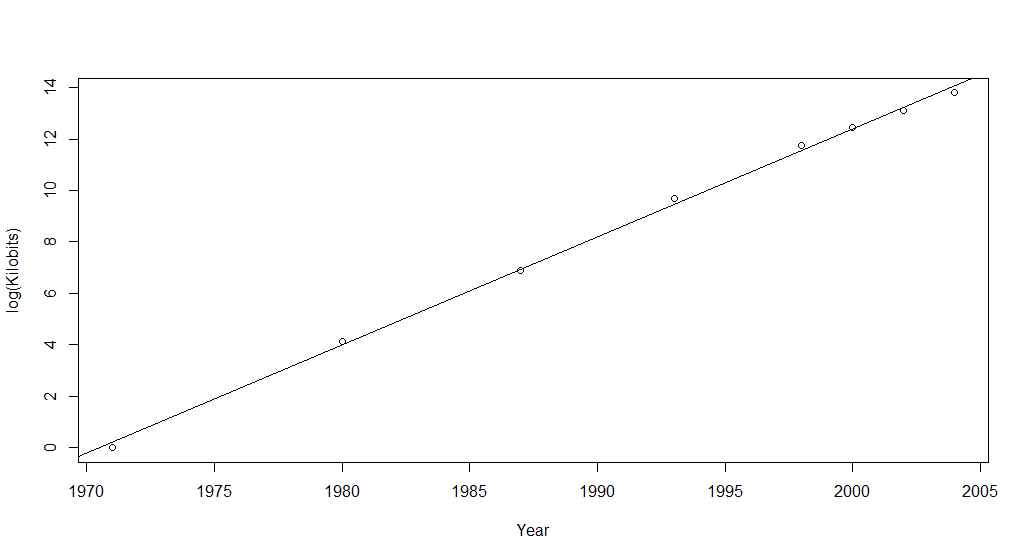
\includegraphics[scale=.5]{hw-10-2-d}

  (e) For $\ln(y)=\beta_0+\beta_1x+\epsilon$
  \begin{enumerate}
    \item Test $H_0: \beta_1=0$ vs. $H_a:\beta_1>0$
    \item Level $\alpha=0.02$
    \item Test statistic $t=\frac{b_1}{SE_{b_1}}$
  \end{enumerate}

  \begin{lstlisting}[backgroundcolor = \color{lightgray},language = R]
    SSE=sum(lmLnKilo$residuals^2)
    [1] 0.2438324
  \end{lstlisting}

  \begin{align*}
    SSE &= \sum(\ln(y_i)-\hat{\ln(y_i)})^2 = 0.2438324\\
    s &= \sqrt{\frac{SSE}{n-2}} = 0.2015905\\
    s_x &= 11.6795 \implies SE_x=11.6795/\sqrt{8} = 4.129327\\
    s_{\ln(y)} &= 4.909217 \implies SE_{\ln(y)}=4.909217/\sqrt{8} = 1.73567\\
    SE_{b_1} &= \frac{s}{s_x\sqrt{n-1}}
      = \frac{0.2015905}{4.129327(7)}
      \approx 0.006974173
  \end{align*}
  
  Therefore the test statistic, 
  $$t=\frac{0.4200238}{0.006974173} \approx \boxed{60}$$

  The critical value at $\alpha=0.02, df=n-p-1=6$ such that $P(T>t^*)=\alpha$.
  $$\implies \boxed{t^*=2.612}.$$

  Since $t>t^*$, we \textbf{fail to reject $H_0$}.\\
\end{solution}

\begin{problem}cheese.txt
\end{problem}
\begin{solution}(a)
  \begin{lstlisting}[backgroundcolor = \color{lightgray},language = R]
    > lmTaste=lm(taste~acetic+h2s+lactic, data=cheese)
    > lmTaste$coefficients
    (Intercept)      acetic         h2s      lactic 
      -9.343375   -2.914695    3.571019   20.139395 
  \end{lstlisting}
  The equation of the least-square regression line based on 
  \textit{Acetic}($x_1$), \textit{H2S}($x_2$) and \textit{Lactic}($x_3$) is
  $$\hat{y}=-9.343375 - 2.914695(x_1) + 3.571019(x_2) + 20.139395(x_3)$$

  (b)
  \begin{lstlisting}[backgroundcolor = \color{lightgray},language = R]
    SSE=sum(lmTaste$residuals^2)
    [1] 3736.907
  \end{lstlisting}
  
  \begin{tabular}{l|l|l}\hline
    Variable & Estimate & SE\\\hline
    Intercept($b_0$) & -9.343 & 22.617\\
    Acetic($b_1$) & -2.915 & 4.754\\
    H2s($b_2$) & 3.571 & 1.341\\
    Lactic($b_3$) & 20.139 & 9.454
  \end{tabular}

  \begin{align*}
    SSE &= \sum(y_i)-\hat{y_i})^2 = 3736.907\\
    s &= \sqrt{\frac{SSE}{n-2}} = 11.55253\\
    s_{x_1} &= 11.6795 \implies SE_x=11.6795/\sqrt{8} = 4.129327\\
    SE_{b_1} &= \frac{s}{s_x\sqrt{n-1}}
    = \frac{0.2015905}{4.129327(7)}
    \approx 0.006974173
  \end{align*}
  
  Test for \textit{Acetic} ($x_1$):
  \begin{enumerate}
    \item Test $H_0: \beta_1=0$ vs. $H_a:\beta_1 \ne 0$
    \item Level $\alpha=0.05$
    \item Test statistic:
    $$
      t = \frac{b_1}{SE_{b_1}}
      = \frac{-2.915}{4.754}
      \approx -0.6132
    $$
    \item Critical Value at $\alpha/2=0.025$
    and Degrees of Freedom, $df=n-4=26$ is
    \begin{lstlisting}[backgroundcolor = \color{lightgray},language = R]
      > qt(1-0.025, 26)
      [1] 2.055529
    \end{lstlisting}
    $$t^*=2.055529$$
    \item We \textbf{fail to reject} $H_0$ since $\abs{t}<t^*$.
  \end{enumerate}
  
  (c) New model for predicting Taste based only on the
      explanatory variables H2S and Lactic:
  \begin{lstlisting}[backgroundcolor = \color{lightgray},language = R]
    > lmTaste2=lm(taste~h2s+lactic, data=cheese)
    > lmTaste2$coefficients
    (Intercept)         h2s      lactic 
     -21.392926    3.193556   18.791786 
  \end{lstlisting}
  The equation of the least-square regression line based on 
  \textit{H2S}($x_2$) and \textit{Lactic}($x_3$) is
  $$\hat{y}=-21.392926 - 3.193556(x_2) + 18.791786(x_3)$$
\end{solution}

\pagebreak

\section*{Project details}
\subsection*{Introduction}
According to the World Health Organization (WHO) stroke is the 2nd leading cause of death globally, 
responsible for approximately 11\% of total deaths. This dataset is used to predict whether a patient
is likely to get stroke based on the input parameters like gender, age, various diseases, and smoking 
status. We can use this dataset to state hypotheses of correlation between various explanatory
variables (like, age, bmi, marital status, residence type, etc.) and the result that they have had
a stroke.\\
The dataset used here can be found on Kaggle, a public competetion forum
where data scientists and novices collaborate to find answers in complex datasets
(\cite{kaggle}). This dataset contains $5110$ data points with $12$ variables:
\begin{enumerate}
  \item \textbf{id:} unique identifier
  \item \textbf{gender:} "Male", "Female" or "Other"
  \item \textbf{age:} age of the patient
  \item \textbf{hypertension:} 0 if the patient doesn't have hypertension, 1 if the patient has hypertension
  \item \textbf{heart\_disease:} 0 if the patient doesn't have any heart diseases, 1 if the patient has a heart disease
  \item \textbf{ever\_married:} ``No'' or ``Yes''
  \item \textbf{work\_type:} ``children'', ``Govt\_jov'', ``Never\_worked'', ``Private'' or ``Self-employed''
  \item \textbf{Residence\_type:} "Rural" or "Urban"
  \item \textbf{avg\_glucose\_level:} average glucose level in blood
  \item \textbf{bmi:} body mass index
  \item \textbf{smoking\_status:} "formerly smoked", "never smoked", "smokes" or "Unknown"*
  \item \textbf{stroke:} 1 if the patient had a stroke or 0 if not
\end{enumerate}

\subsection*{Methods}
According to stroke.org, a non-profit organization dedicated to public awareness about,
and prevention of common causes of stroke, smoking, lack of physical activity, diabetes and 
obesity are leading factors that could lead to stroke (\cite{strokeorg}).
In particular we explore the following question\\

\fbox{Is BMI correlated to any other ``quantitative'' value?}\\

We start with analysing the ``class'' of each variable:
\begin{lstlisting}[backgroundcolor = \color{lightgray},language = R]
  > sapply(stroke, class)
  id              gender            age           hypertension
  "integer"       "factor"          "numeric"     "integer"
  heart_disease   ever_married      work_type 
  "integer"       "factor"          "factor" 
  Residence_type  avg_glucose_level bmi
  "factor"        "numeric"         "factor"
  smoking_status  stroke 
  "factor"        "integer" 
\end{lstlisting}
Since ``bmi'' is the quantity we're interested in, we notice that 
it is listed as ``factor'' and not ``numeric''. This is because
there are values like ``N/A'' for some items. We filter those out:
\begin{lstlisting}[backgroundcolor = \color{lightgray},language = R]
  > stroke2=stroke[stroke$bmi!='N/A',]
  > stroke2=transform(stroke2, bmi=as.numeric(bmi))
  > dim(stroke2)
  [1] 4909   12
\end{lstlisting}
Now the interesting ``numeric'' variables are
\textbf{Age} and \textbf{Average glucose level}

At this point we can plot ``bmi''
against each of these variables\\
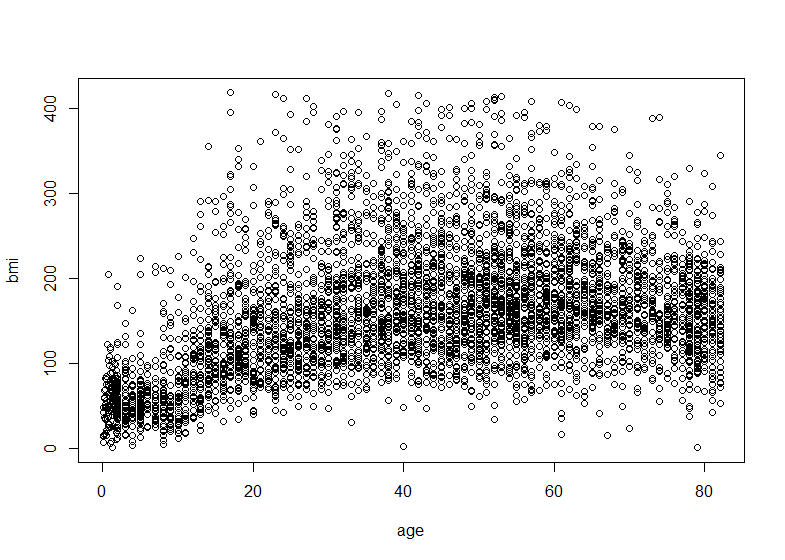
\includegraphics[scale=.5]{bmi-age}\\
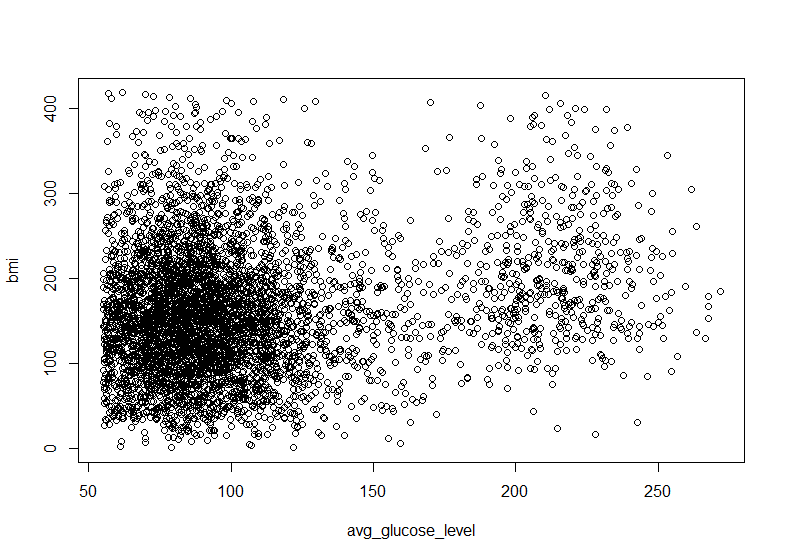
\includegraphics[scale=.5]{bmi-avg_glucose_level}\\

And build a linear-regression model
\begin{lstlisting}[backgroundcolor = \color{lightgray},language = R]
  > lmStroke=lm(bmi~age+avg_glucose_level, data=stroke2)
  > lmStroke$coefficients
  (Intercept)     age(x1)       avg_glucose_level (x2)
  96.902336       1.080037      0.179388 
\end{lstlisting}
Therefore the equation of the least-square regression line is
$$ \hat{y} = 96.902336 + 1.080037(x_1) + 0.179388(x_2) $$

\begin{tabular}{l|l|l}\hline
  Variable & Estimate & SE\\\hline
  Intercept & 96.90234 & 2.91577\\
  Age & 1.08004 & 0.04556\\
  Avg glucose level & 0.17939 & 0.02313
\end{tabular}

\subsection*{Next steps}
\begin{enumerate}
  \item Make hypotheses for ``age'' and ``average glucose level''
  \item Calculate test statistics for each of these hypotheses
  \item Conclude whether the hypotheses can or cannot be rejected
\end{enumerate}
\pagebreak
\printbibliography

\end{document}
